
\label{cha:PIC - Code}
\section{PIC-Code}
\pra

\subsection{Definition}

 Die Sprache \textit{PIC-Code} ist eine Erweiterung von \verb|troff|. Das Textsatzsystem \verb|troff| erlaubt dem Benutzer einen qualitativ hochwertigen Text zu erstellen oder ein Diagramm zu zeichnen, wofür jedoch Erweiterungen benötigt werden.\footfullcite[][]{Making_Pictures_With_GNU} PIC stellt zusätzlich Features zur Verfügung, mit welchen zum Beispiel Boxen, Linien oder Ellipsen einfach dargestellt und verbunden werden können.
\\

\noindent
Falls in einem \verb|troff|-Dokument beispielsweise ein Diagramm gezeichnet werden soll, ist dies ohne weitere Extras nicht möglich. Um dies umzusetzen, kann \textit{PIC} in den Code eingebunden werden. Mithilfe der Erweiterung sollte es nun möglich sein, das gewünschte Objekt zu generieren, da \textit{PIC} die Möglichkeiten bietet, Gegenstände zu zeichnen, zu verbinden oder zu färben. \footnotemark[13]

\subsection{Aufbau einer PIC Datei}
\pra
\noindent
Der Aufbau einer PIC-Datei wird in Listing \ref{PIC-Aufbau-list}\footnotemark[13] veranschaulicht:
\noindent
\lstset{frame=lines}
\lstset{caption={Beispielaufbau einer PIC-Datei}}
\lstset{label={PIC-Aufbau-list}}
\lstset{basicstyle=\footnotesize}
\begin{lstlisting}
.PS
ellipse "document";
arrow;
box "\fIpic\fP(1)"
arrow;
box width 1.2 "\fIgtbl\fP(1) or \fIgeqn\fP(1)" "(optional) dashed;
arrow;
box "\fIgtroff\fP(1)";
arrow;
ellipse "PostScript";
.PE

\end{lstlisting}
 Der Aufbau von jedem \textit{PIC} Programm ist im Prinzip gleich. Jede Datei muss zu Beginn des Codes ein \verb|.PS| stehen haben, da dies dem Compiler kennzeichnet, dass ab diesem Zeitpunkt Befehle in der Sprache \textit{PIC} zu erwarten sind. Falls der Eintrag \verb|.PS| fehlt, so gibt der Compiler während des Ausführens einen Syntax-Fehler aus und weist darauf hin, dass der erforderliche Ausdruck fehlt.
\\

\noindent
Das Ende eines \textit{PIC} Programmcodes ist mittels \verb|.PE| gekennzeichnet. Das Fehlen dieses Eintrages trägt dazu bei, dass der Compiler kein Ende der Datei vorfindet und es tritt ebenfalls ein Syntaxfehler auf.
\\

\noindent
Die Ausgabe des oben gezeigten Codes sieht wie folgt aus (Abbildung \ref{Erg_Beispielcode_1})\footnotemark[13]:
\\
\begin{figure}[H]
	\begin{center}
		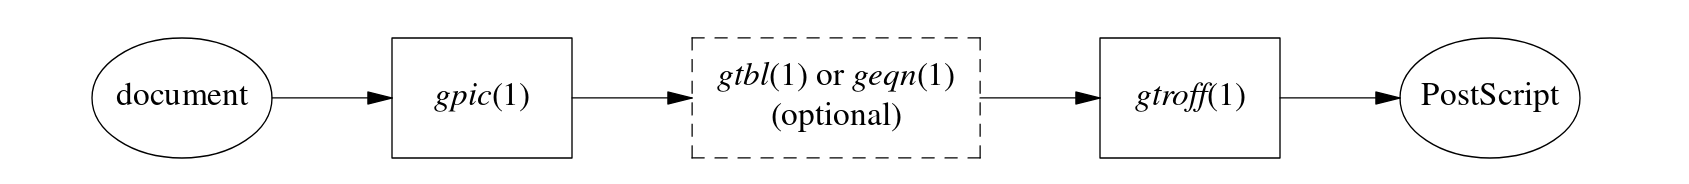
\includegraphics[width=13cm]{images/Ergebnis_1.png}
		\caption{Erzeugter Graph des Beispielcodes}
		\label{Erg_Beispielcode_1}
	\end{center}
\end{figure}

\subsection{Objekte zeichnen in PIC}

\noindent
In \textit{PIC-Code} ist es möglich verschiedene Objekte zu zeichnen. Hierbei gibt es vordefinierte Objekte, jedoch können auch neue Objekte generiert werden.
\\

\noindent
Abbildung \ref{Objekte_PIC} \footfullcite[][]{Making_Pictures_With_GNU} zeigt die grundsätzlichen Objekte von PIC:
\\
\begin{figure}[H]
	\begin{center}
		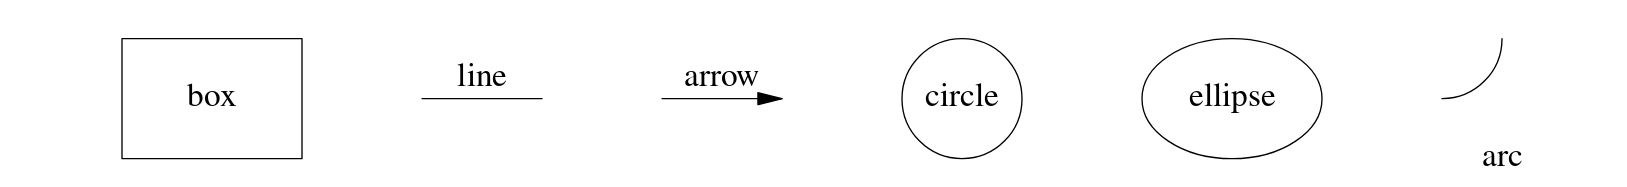
\includegraphics[width=13cm, height=2cm]{images/Objekte_PIC.png}
		\caption{Vordefinierte Objekte}
		\label{Objekte_PIC}
	\end{center}
\end{figure}

\pra

\noindent
Die Form einer Raute ist standardmäßig nicht definiert, lässt sich jedoch leicht implementieren. Es besteht nämlich die Möglichkeit, den Rand der Raute mit Hilfe von verbundenen Linien zu zeichnen. Listing \ref{list-raute} veranschaulicht die Generierung einer Raute:
\\
\noindent
\lstset{frame=lines}
\lstset{caption={Code zum Zeichnen einer Raute}}
\lstset{label={list-raute}}
\lstset{basicstyle=\footnotesize}
\begin{lstlisting}
.PS
box invis;
line from last box .n to last box .e then
to last box .s then to last box .w then to
last box .n
.PE
\end{lstlisting}

\noindent
Die generierte Raute ist in Abbildung \ref{Diamant_PIC} zu sehen.
\\
\begin{figure}[H]
	\begin{center}
		
\includegraphics[width=13cm]{images/Diamant_Beispiel.png}
		\caption{Gezeichnete Raute aus dem obigen Codebeispiel}
		\label{Diamant_PIC}
	\end{center}
\end{figure}

\noindent
\textit{PIC} verfügt über eine große Auswahl an Möglichkeiten, um ein bestimmtes Objekt zu zeichnen. Man kann durch zusätzliche Argumente zum Beispiel die Breite und die Höhe einer Box festlegen, ob der Rahmen eine durchgezogene Linie oder nur strichliert dargestellt werden soll oder ob die Box in einer bestimmten Farbe zu generieren ist. 
\\
\pra
\noindent
Der benötigte Code, um eine gelbe Ellipse zu zeichnen, wird in Listing \ref{list-Ellipse-gelb} dargestellt: 
\\
\noindent
\lstset{frame=lines}
\lstset{caption={PIC-Code zum Zeichnen einer gelben Ellipse}}
\lstset{label={list-Ellipse-gelb}}
\lstset{basicstyle=\footnotesize}
\begin{lstlisting}
.PS
ellipse shaded "yellow";
.PE
\end{lstlisting}

\noindent
Die gefärbte Ellipse wird in Abbildung \ref{Ellipse_Gelb} veranschaulicht:
\\
\begin{figure}[H]
	\begin{center}
		
\includegraphics[width=8cm]{images/Ellipse_Beispiel.png}
		\caption{Gelbe Ellipse}
		\label{Ellipse_Gelb}
	\end{center}
\end{figure}
\pra
\noindent
In \textit{PIC-Code} sind standardmäßig einige Farben vordefiniert. Es besteht jedoch auch die Möglichkeit, Farben mittels zum Beispiel hexadezimalen Werten zu definieren. Die Farbwerte können ebenfalls mit Hilfe von dem \textit{RGB}-Modell angegeben werden. Um eine neue Farbe in \textit{PIC-Code} zu definieren wird folgender Code benötigt (Listing \ref{list-farbe-def}):
\\

\noindent
\lstset{frame=lines}
\lstset{caption={Code zum Definieren einer neuen Farbe}}
\lstset{label={list-farbe-def}}
\lstset{basicstyle=\footnotesize}
\begin{lstlisting}
.PS
.defcolor medblue rgb #89D8D6
.PE
\end{lstlisting} 

\noindent
Die definierte Farbe \verb|medblue| kann so wie jede andere Farbe normal verwendet werden. Listing \ref{use-farbe} zeigt einen Beispielaufruf:
\\
\noindent
\lstset{frame=lines}
\lstset{caption={Anwendung der neu definierten Farbe}}
\lstset{label={use-farbe}}
\lstset{basicstyle=\footnotesize}
\begin{lstlisting}
.PS
    box shaded medblue;
.PE
\end{lstlisting}

\noindent
Der Code liefert als Ergebnis eine Box in einem helleren Blauton. Die Grafik wird in Abbildung \ref{Farbe_def} veranschaulicht.
\\ 
\begin{figure}[H]
	\begin{center}
		
\includegraphics[width=3.5cm]{images/Box_Medblue.png}
		\caption{Box in der selbst definierten Farbe \textit{medblue}}
		\label{Farbe_def}
	\end{center}
\end{figure}
\noindent
\pra
In \textit{ERDs} müssen unter anderem auch \textit{abhängige Entitytypen} gezeichnet werden. Diese werden dargestellt, indem die Umrandung des Objektes doppelt gezeichnet wird. Das betrifft Entities und Beziehungen. 
\\

\noindent
Der Code für eine Box mit doppelt gezeichneten Linien sieht wie folgt aus(Listing \ref{list-doppelt-box}):
\\
\noindent
\lstset{frame=lines}
\lstset{caption={PIC-Code für eine Box mit doppelter Umrandung}}
\lstset{label={list-doppelt-box}}
\lstset{basicstyle=\footnotesize}
\begin{lstlisting}
.PS
boxht=1;boxwid=1;box at (0, 0);
boxht=1.2;boxwid=1.2; box at (0, 0);
.PE
\end{lstlisting}

\noindent
Abbildung \ref{Box_doppelt} zeigt das Ergebnis des oben angeführten Codes. 
\\
\begin{figure}[H]
	\begin{center}
		
\includegraphics{images/Box_doppelt.png}
		\caption{Box mit doppelter Umrandung}
		\label{Box_doppelt}
	\end{center}
\end{figure}

\noindent
Für die Implementierung einer abhängigen Beziehung werden zwei Rauten übereinander gezeichnet, wobei eine der beiden Rauten über eine größere Höhe und Breite verfügt. In der Praxis sieht der generierte \textit{PIC-Code} wie folgt aus (siehe Listing \ref{list-doppelt-raute}):
\\
\noindent
\lstset{frame=lines}
\lstset{caption={PIC-Code zur Generierung einer Raute mit doppelter Umrandung}}
\lstset{label={list-doppelt-raute}}
\lstset{basicstyle=\footnotesize}
\begin{lstlisting}
.PS
boxht=1;boxwid=1;box invis at (0, 0);
line from last box .n to last box .e then to last box .s
then to last box .w then to last box .n;
boxht=1.2;boxwid=1.2; box invis at (0, 0);
line from last box .n to last box .e then to last box .s
then to last box .w then to last box .n;
.PE
\end{lstlisting}

\pra
\noindent
Aus diesem Code wird folgende Grafik erstellt(siehe Abbildung \ref{Raute_doppelt}):
\\

\begin{figure}[H]
	\begin{center}
		
\includegraphics{images/Raute_doppelt.png}
		\caption{Raute mit doppelter Umrandung}
		\label{Raute_doppelt}
	\end{center}
\end{figure}

\noindent
Für die Implementierung einer \textit{Super/Sub}-Beziehung muss die Form eines Dreiecks gezeichnet werden. Der benötigte Code wird in Listing \ref{dreieck-list} gezeigt:
\pra
\noindent
\lstset{frame=lines}
\lstset{caption={PIC-Code zum Zeichnen eines Dreiecks}}
\lstset{label={dreieck-list}}
\lstset{basicstyle=\footnotesize}
\begin{lstlisting}
.PS
box invis;
line from last box .n to last box .se then to last box .sw
then to last box .n
.PE
\end{lstlisting}
\noindent
Listing \ref{dreieck-list} hat folgende Ausgabe (siehe Abbildung \ref{Dreieck}) :
\\

\begin{figure}[H]
	\begin{center}
		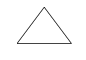
\includegraphics{images/Dreieck.png}
		\caption{gezeichnetes Dreieck von dem abgebildeten Code}
		\label{Dreieck}
	\end{center}
\end{figure}
\pra
\noindent
Ein Feature von \textit{PIC}-Code ist, dass man mit Labels arbeiten kann. Darunter versteht man, dass Objekten eine bestimmte ID zugewiesen werden kann, um im nachhinein einfach darauf zuzugreifen. Dies kann unter anderem nützlich sein, wenn zwei bestimmte Elemente verbunden werden sollen, die nicht direkt nacheinander gezeichnet wurden. Dabei sind gewisse Syntaxregeln für ein Label einzuhalten. Es darf nämlich keine Leerzeichen enthalten und muss mit einem Großbuchstaben beginnen. Weiters dürfen keine Ziffern und Umlaute vorkommen. 
\\
\pra
\noindent
\lstset{frame=lines}
\lstset{caption={Objekte mit Labels versehen und verbinden}}
\lstset{label={list-label}}
\lstset{basicstyle=\footnotesize}
\begin{lstlisting}
.PS
A: box;
move;
B: circle;
down;
move;
C: ellipse;
line from A to C;
.PE
\end{lstlisting}

\noindent
Das entstandene Bild aus Listing \ref{list-label} \footfullcite[][]{Making_Pictures_With_GNU} ist in Abbildung \ref{Label} \footnotemark[15] zu sehen.
\\

\noindent
\begin{figure}[H]
	\begin{center}
		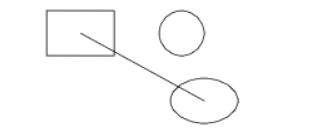
\includegraphics[width=7cm]{images/Ergebnis_Label.png}
		\caption{Objekte mit Labels versehen und verbinden}
		\label{Label}
	\end{center}
\end{figure}

\pra
\noindent
Um das Layout der gezeichneten Elemente zu bestimmen, gibt es mehrere Methoden. Wenn keine zusätzlichen Befehle angegeben werden, generiert \textit{PIC} das erste Objekt in der linken oberen Ecke des Bildes und fügt die restlichen rechts daneben ein. Es gibt jedoch die Möglichkeit, das Layout der generierten Datei mittels Addieren oder Subtrahieren der Koordinaten zu verändern und somit den Standort der Graphen zu bestimmen. Eine weitere Art der Spezifizierung kann dadurch erreicht werden, indem x- und y-Werte direkt in den Befehl eingebunden werden. In Listing \ref{list-kord} ist ein Beispiel abgebildet, wie Objekte an bestimmten Koordianten gezeichnet werden.
\\

\noindent
\lstset{frame=lines}
\lstset{caption={PIC-Code zur Generierung einer Box an den Koordinaten [100, 100]}}
\lstset{label={list-kord}}
\lstset{basicstyle=\footnotesize}
\begin{lstlisting}
.PS
A:box at (100, 100);
.PE
\end{lstlisting}

\noindent
Um den \textit{Primary Key} von einem \textit{Entity} zu bestimmen, muss der Inhalt des \textit{Primary-Key}-Attributes unterstrichen werden. Dies wird in \textit{PIC}-Code implementiert, indem 2 Ellipsen übereinander gezeichnet werden, wobei in einer Ellipse der Name des \textit{Attributes} steht und in der zweiten Ellipse befinden sich anstatt eines Textes als Name mehrere aufeinanderfolgende Unterstriche. Der Code, um dieses Ergebnis zu erzielen, wird in Listing \ref{list-unter} veranschaulicht:
\pra
\lstset{frame=lines}
\lstset{caption={PIC-Code zum Unterstreichen von Text in einer Ellipse]}}
\lstset{label={list-unter}}
\lstset{basicstyle=\footnotesize}
\begin{lstlisting}
.PS
ellipse "Unterstrichen";
ellipse at last ellipse "__________";
.PE
\end{lstlisting}

\noindent
Aus Listing \ref{list-unter} wird folgende Grafik erzeugt (siehe Abbildung \ref{Unterstrichen})):

\noindent
\begin{figure}[H]
	\begin{center}
		
\includegraphics[width=3.5cm]{images/Ellipse_unterstrichen.png}
		\caption{Text der Ellipse wird unterstrichen}
		\label{Unterstrichen}
	\end{center}
\end{figure}

\noindent
Weiters müssen die \textit{Primary Keys} von \textit{abhängigen Entities} mit einer strichlierten Linie unterstrichen werden. Der \textit{PIC-Code} zur Darstellung eines Attributes mit einem strichliert unterstrichenem Text sieht wie folgt aus (Listing \ref{list-unterstr}):

\lstset{frame=lines}
\lstset{caption={Text der Ellipse wird strichliert unterstrichen}}
\lstset{label={list-unterstr}}
\lstset{basicstyle=\footnotesize}
\begin{lstlisting}
.PS
ellipse "Unterstrichen";
ellipse at last ellipse "_ _ _ _ _ _";
.PE
\end{lstlisting}

\noindent
Der in Listing \ref{list-unterstr} gezeigte Code generiert folgende Grafik (siehe Abbildung \ref{strichl_unter}):
\begin{figure}[H]
	\begin{center}
		
\includegraphics[width=3.5cm]{images/Ellipse_strichliert.png}
		\caption{Text der Ellipse wird strichliert unterstrichen dargestellt}
		\label{strichl_unter}
	\end{center}
\end{figure}

\subsubsection{Anpassen der Objekte}
\pra

\noindent
In \textit{PIC}-Code steht die Option zur Verfügung, dass Eigenschaften von Objekten wie zum Beispiel von Boxen, Ellipsen oder von Kreisen per Hand hinzugefügt werden können. Dies betrifft unter anderem die Höhe und die Breite. Weiters können Attribute für das ganze Dokument angegeben werden, wie zum Beispiel die maximale Höhe und Breite von dem gesamten Bild. Standardmäßig sind diese Werte bei Boxen und Ellipsen 0.5 cm und 0.75 cm. Der Radius für einen Kreis beträgt 0.25 cm, falls dieser nicht angegeben wird. 
\\

\noindent
Um die Breite und die Höhe beispielsweise auf jeweils 4 Zentimeter zu setzen, muss der Code wie folgt aussehen (siehe Listing \ref{list-wid-ht}):

\lstset{frame=lines}
\lstset{caption={Setzen der Boxbreite und -höhe auf 4cm}}
\lstset{label={list-wid-ht}}
\lstset{basicstyle=\footnotesize}
\begin{lstlisting}
.PS
quadrat: boxwid=4;boxht=4; box;
.PE
\end{lstlisting}

\noindent
Es gibt ausserdem die Option, ein bestimmtes Objekt zu skalieren. Diese kann hilfreich sein, wenn die Grenzen des zu generierenden Bildes sehr groß sind. Listing \ref{list-scale} zeigt, wie der Skalierungsfaktor einer Box gesetzt werden kann:

\lstset{frame=lines}
\lstset{caption={Setzen des Skalierungsfaktors einer Box auf 15}}
\lstset{label={list-scale}}
\lstset{basicstyle=\footnotesize}
\begin{lstlisting}
.PS
scaledbox: scale=15; box;
.PE
\end{lstlisting}

\subsection{Layout}
\label{layout}
\pra
\noindent
Das Layout des ganzen Diagrammes wird mit Hilfe von \verb|graphviz-layout| erzeugt. 

\noindent
Der Python-Code für die Generierung der Koordinaten wird in Listing \ref{list-python-layout} gezeigt:
\\
\lstset{language=Python}
\lstset{frame=lines}
\lstset{caption={Python Code zur Generierung des Layouts mittels graphviz-layout}}
\lstset{label={list-python-layout}}
\lstset{basicstyle=\footnotesize}
\begin{lstlisting}
def nx_graph(rel):
    erd = nx.Graph()
    for curr in rel:
        if len(curr) > 1:
            for i in range(len(curr)):

                erd.add_edge(curr[0], curr[i])
        else:
            continue
    pos = graphviz_layout(erd, prog='neato', args="-Gsplines=true -Goverlap=scale -Gsize=100,200! -Gmaxiter=10000 -Gepsilon=0.00001 -Gdpi=1 -Gratio=fill" )
    return pos
\end{lstlisting}

\noindent
Der Befehl \verb|graphviz_layout| verfügt über einige Parameter, die das zu generierende Layout bestimmen. Das Argument \verb|prog| gibt den Algorithmus für das Layout an. Als gültige Parameter dieses Arguments gelten \footfullcite{graphviz_visualization}: 
\\

\begin{itemize} \pra 
	\item{\verb|dot|} kann sinnvoll verwendet werden, wenn das gewünschte Ergebnis hierarchisch oder geschichtet dargestellt werden soll.
	\item{\verb|neato|} produziert die Grafik gemäß des \textit{Sprungfedermodells}. Dieser Parameter ist der Standard für ungerichtete Graphen.
	\item{\verb|twopi|} erstellt für gerichtete und ungerichtete Graphen eine Darstellung, bei der die Knoten radial angeordnet werden.
	\item{\verb|fdp|} beinhaltet einen Mehrgitterlöser zur Behandlung von großen und geclusterten Graphen.
	\item{\verb|sfdp|} ist eine skalierbare Version von \verb|fdp|. Diese Option eignet sich besonders gut für große Diagramme.
	\item{\verb|circo|} ordnet die Knoten kreisförmig an. Dieser Parameter erweist sich als sinnvoll für bestimmte Diagramme von mehrfach zyklischen Strukturen.
\end{itemize}

\noindent
Jeder dieser Layoutalgorithmen hat seine Vorteile, jedoch bietet \verb|neato| angewendet auf alle Datenmodelle das bestgeeignetste Layout für ein \textit{Entitiy Relationship Diagramm} mit den wenigsten Überschneidungen der Linien.
\\

\noindent
Es können weitaus mehr Layoutalgorithmen angegeben werden, jedoch sind die oben aufgezählten Parameter am Sinnvollsten beziehungsweise erstellen diese Algorithmen ein \textit{Entity Relationship Diagramm} in einem gut lesbaren Layout. 
\\

\noindent
Die Argumente des Parameters \verb|args| sind Zusatzeinstellungen, die für die Generierung der Grafik nützlich sind. Unter anderem kann als Attribut \verb|-Gsize| angegeben werden um die Größe des Dokuments zu bestimmen. Weitere Argumente sind zum Beispiel \verb|-Gsplines|
\verb|-Goverlap, -Gmaxiter, -Geplsilon, -Gdpi| und \verb|-Gratio|.
\\

\subsection{Erstellen einer PIC-Datei}
\pra

\noindent
Der \textit{Python}-Code, indem die \textit{PIC}-Datei erstellt und beschrieben wird, sieht wie folgt aus (Listing \ref{list-pic-file}):

\lstset{language=Python}
\lstset{frame=lines}
\lstset{caption={Python Code, indem der generierte PIC-Code in eine selbsterstellte PIC-Datei geschrieben wird}}
\lstset{label={list-pic-file}}
\lstset{basicstyle=\footnotesize}
\begin{lstlisting}
def write_erd_to_file(pic):

    if os.path.exists("erd.pic"):
        os.remove("erd.pic")
    file = open("erd.pic", "w")
    file.write(pic)  
    file.close()
    print('Your file is created at: ' + os.getcwd() + '/erd.pic')

\end{lstlisting}

\noindent
Der Parameter \textit{pic} ist der generierte \textit{PIC}-Code, der das \textit{ERD} zeichnet.

\noindent
Sobald in das erstellte Dokument der \textit{PIC}-Code ergänzt wurde, kann die Datei kompiliert und angezeigt werden.

\subsection{Vorteile und Nachteile von PIC}
\pra

\subsubsection{Vorteile}

\noindent
Die Erweiterung \textit{PIC} bietet einige Vorteile, die für die Generierung von Dokumenten und Graphen hilfreich sein können:
\\
\begin{itemize}
	\item Da die Sprache sehr einfach aufgebaut ist und die Namen der Befehle bzw. Objekte sprechend gewählt wurden, fällt es einem späteren Leser nicht schwer, den Code zu verstehen. Vor allem mit Hilfe der vordefinierten Objekte wird das Generieren grundlegender Graphen um einiges vereinfacht und erfordert keinen großen Aufwand.
	\lstset{frame=lines}
	\lstset{caption={Leicht lesbarer Code zur Generierung einer Grafik}}
	\lstset{label={list-corde-lesbar}}
	\lstset{basicstyle=\footnotesize}
	\begin{lstlisting}
.PS
box "from"
move 0.75;
ellipse "to";
arc cw from 1/3 of the way \
 between last box .n and last box .ne to last ellipse .n;
.PE
	\end{lstlisting}
	
	\noindent
	Aus Listing \ref{list-corde-lesbar}\footfullcite[][]{Making_Pictures_With_GNU} wird folgende Grafik erzeugt(sieht Abbildung \ref{SprechendName} \footnotemark[17]):
	\begin{figure}[H]
		\begin{center}
			
\includegraphics[width=13cm]{images/PIC_Aufbau_Einfachkeit.png}
			\caption{Ergebnis des Codes}
			\label{SprechendName}
		\end{center}
	\end{figure}
	
	\item Weiters kann man dank der Fehlermeldungen und des leicht zu lesenden Codes sowohl syntaktische als auch logische Fehler ohne großem Aufwand finden und beheben.


\end{itemize}

\subsubsection{Nachteile}
\pra

\noindent
Neben den Vorteilen gibt es jedoch auch Nachteile, die im Vergleich zu den Pro-Argumenten überwiegen. Zu den negativen Aspekten zählen:

\begin{itemize}
	\item Die Anzahl der standardmäßig definierten Objekte in \textit{PIC} ist nur gering. Daraus folgt, dass der Aufwand andere Objekte zu zeichnen steigt, auch wenn das nur geringfügig bzw. der Code leicht zu generieren ist. \textit{PIC} verfügt zwar über die Möglichkeit, Makros zu definieren, jedoch ist die Definition dieser Makros ein Aufwand, der bei den anderen Implementierungsvarianten nicht existiert, da dort die benötigten Objekte bereits vordefiniert sind.
	\\
	\pra
	\item Weiters ist über \textit{PIC}-Code zu sagen, dass das Verbinden von zwei unterschiedlichen Objekten in der Theorie recht einfach ist, praktisch jedoch nur mit viel Aufwand verbunden umgesetzt werden kann. Es müssen nämlich die Bezugspunkte (Norden, Osten, Süden, Westen) angegeben werden, denn ohne diese Information befinden sich der Beginn und das Ende der gezeichneten Linie in der Mitte des jeweiligen Objektes. Falls dieser Gegenstand eine Beschriftung aufweist, hat dies zur Folge, dass der Inhalt der Box schwerer bis nicht mehr lesbar wird. Dies ist insofern ein Nachteil, da das Verbinden der Objekte viele Abfragen benötigt, weil der Start- und der Endpunkt nicht sofort bekannt sind. Die Koordinaten der zwei zu verbindenden Elemente müssen zuerst verglichen werden, um dann die richtigen Bezugspunkte zu wählen. 
	Ohne diese Abfragen sieht die Verbindung zwischen zwei Boxen aus wie in Abbildung \ref{ConnProb} zu sehen ist.
	\begin{figure}[h!]
		\begin{center}
			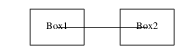
\includegraphics[width=7cm]{images/Connectoren_Problem.png}
			\caption{Konnektoren ohne zusätzlicher Information über Start- und Endpunkt}
			\label{ConnProb}
		\end{center}
	\end{figure}

	\noindent
	\textit{PIC}-Code unterscheidet sich in diesem Punkt von \textit{Graphviz, Libre Office Draw} und \textit{Graphml}. Bei den Varianten werden die Bezugspunkte automatisch gesetzt.
	\\
	
	\item 
	Die Generierung des Layouts des ganzen Diagrammes stellt generell ein großes Problem dar. Mittels \textit{PIC}-Code ist es nicht möglich, ein gut aussehendes \textit{ERD} zu erzeugen. Daher muss mit Hilfe von \textit{Graphviz} das Layout im vorhinein generiert werden, wobei nur die Koordinaten der Knoten erzeugt werden und nicht das ganze Diagramm. Ausgehend von diesen Werten können dann die Objekte einfach im \textit{PIC}-Code positioniert werden (siehe Kapitel \ref{layout}). 
	\pra
	\noindent
	Auf Grund dieser Methode tritt ein weiteres Problem auf und zwar, dass man beim Generieren der Koordinaten die richtigen Parameter für den Befehl \verb|graphviz_layout| benötigt. Diese müssen mit dem Dokument übereinstimmen, da sonst die Werte der Koordinaten zu groß werden und deswegen Elemente ausserhalb des Dokuments gezeichnet werden. Ausserdem erzeugt dieser Befehl die generierten Punkte in einem viel zu großen Ausmaß, sodass die Werte trotz richtigen Parametern noch bearbeitet werden müssen.
	\\
	
	\item Bei der Generierung des Layouts treten häufig Probleme auf. Das liegt daran, dass PIC die Koordinaten in \textit{inches} berechnet, jedoch eine PDF Datei mit Pixel arbeitet. Dies erschwert das Generieren mittels absoluten Koordinaten, da von PIC nicht überprüft wird, ob der Wert noch innerhalb des anzeigbaren Bereiches liegt oder ob dieser ausserhalb des gegebenen Bereiches gezeichnet wird. Dies kann zur Folge haben, dass ein Objekt teilweise abgeschnitten wird, wie in der Abbildung \ref{Box_Cut} zu sehen ist.
	\\
	
	\lstset{frame=lines}
	\lstset{caption={PIC-Code, um den Fehlerfall zu zeigen, dass eine Box bei zu großen Koordinaten abgeschnitten wird}}
	\lstset{label={list-box-cut}}
	\lstset{basicstyle=\footnotesize}
	\begin{lstlisting}
	.PS
	box at (0, 300);
	.PE
	\end{lstlisting}
	
	\noindent
	Listing \ref{list-box-cut} wird in Abbildung \ref{Box_Cut} veranschaulicht:
	\noindent
	\begin{figure}[H]
		\begin{center}
			
\includegraphics[scale=0.5]{images/Erg_Code_abgeschnitten.png}
			\caption{Box wird wegen zu großen Koordinaten abgeschnitten}
			\label{Box_Cut}
		\end{center}
	\end{figure}
\pra
	Wenn die Koordinaten zu groß werden, kann es auch zu dem Fall kommen, dass diese nicht einmal mehr in der Nähe der maximalen Grenzen liegen. Das hat zur Folge, dass das Element nicht mehr angezeigt werden kann. 
	\\
	\lstset{frame=lines}
	\lstset{caption={Code, um den Fehlerfall zu erzeugen, dass eine Box ausserhalb des sichtbaren Bereiches gezeichnet wird}}
	\lstset{label={list-err}}
	\lstset{basicstyle=\footnotesize}
	\begin{lstlisting}
	.PS
	box at(500, 0)
	boxwid=35;boxht=15;  bot at (0, 0);
	line from 1st box to last box;
	\end{lstlisting}
	\noindent
	Die generierte Grafik wird in Abbildung \ref{Box_Away} verbildlicht. \pra
	\begin{figure}[h!]
		\begin{center}
			
\includegraphics{images/ERG_Box_weg.png}
			\caption{Box wird wegen zu großen Koordinaten ausserhalb des Sichtfeldes gezeichnet}
			\label{Box_Away}
		\end{center}
	\end{figure}
	\\	
\end{itemize}
